\documentclass[11pt]{article}
\usepackage[utf8]{inputenc}
\usepackage[T1]{fontenc}
\usepackage{mathptmx}
\usepackage[margin=1in]{geometry}
\usepackage{microtype}
\usepackage{amsmath}
\usepackage{graphicx}
\usepackage{booktabs}
\usepackage{tabularx}
\usepackage{array}
\usepackage{xcolor}
\usepackage[round,authoryear]{natbib}
\usepackage[hidelinks]{hyperref}
\usepackage{caption}
\captionsetup{font=small,labelfont=bf}
\newcommand{\todo}[1]{\textcolor{red}{[#1]}}

\title{Information Access and Gain-Loss Framing in Six Large Language Models and Human Decision Makers}
\author{
  Aadithya Chandramouli\\
  School of Electrical Engineering and Computer Science\\
  College of Engineering, The Pennsylvania State University
  \and
  Jeremy M. Gernand\\
  College of Earth and Mineral Sciences\\
  The Pennsylvania State University \todo{confirm department}
}
\date{}
\begin{document}
\maketitle
\begin{abstract}
A risky choice can be described by what will be saved or by what will be lost, and people often choose differently depending on that wording. We test whether six large language models (LLMs) from four developers show this gain-loss framing effect, and whether the effect shrinks when the models can read extra information about the options before choosing. GPT-4.1, GPT-4o, GPT-4o-mini, Gemini 2.5 Flash, Qwen3 235B and Llama 4 Maverick made 11,519 choices across four risk scenarios, each presented in its original wording, two paraphrases and a mirrored version with the same facts in the opposite frame. Before choosing, a model could open 0, 2, 3 or 4 of seven information cards. We compare the models with 198 students who did the same card task and chose for themselves how many cards to open. With no cards, all six models showed large framing effects: weighting each topic equally, the share choosing the sure option was 27 to 79 percentage points lower under loss wording than under gain wording. Allowing cards reduced this gap in every model at the 2-card limit, but in the balanced comparison only GPT-4.1 met a prespecified 10-point threshold at 4 cards, the highest limit tested. Qwen3 met it at 2 cards but not at 3 or 4, and no other model met it. GPT-4o-mini and Llama 4 Maverick kept gaps of 28 to 66 points, and for GPT-4o-mini and Qwen3 the gap grew as the card limit rose from 2 to 4. In people, a gap appeared in decisions made after opening 0 or 1 cards and was not detected after opening more, although the human design ties wording to topic and order. Access to more information was associated with smaller framing effects in most models, but the size of the reduction depended on the model, the scenario and how the results are aggregated.
\end{abstract}

\section{Introduction}

The same risky choice can be described in two ways. A response program can save 200 of 600 people for certain, or it can let 400 of 600 people die for certain. The outcomes are identical, yet people tend to prefer the sure option when outcomes are described as gains and to gamble when they are described as losses \citep{tversky1981framing}. This gain-loss framing effect has been replicated many times \citep{kuhberger1998influence}, and biases of this kind matter wherever risks are assessed and communicated \citep{montibeller2015cognitive,gernand2023set}.

As LLMs are used to answer questions and support decisions, it matters whether their choices also depend on wording. \citet{binz2023using} found that GPT-3 showed a framing effect on classic vignettes, and \citet{echterhoff2024cognitive} found a range of cognitive biases, including framing, in LLM decision making. Most such tests give a model a short vignette and ask for a choice. In practice, a person or a model can often read more about each option before deciding.

We ask whether access to option-specific information changes how much the wording matters, and how much access is needed before the difference falls below a practical threshold. People who look at more information before deciding may rely less on the wording, but it is not known whether the same holds for LLMs.

We study this with an information-card task. Each scenario offers a safe and a risky option, worded as either a gain or a loss. Before choosing, the decision maker can open up to a set number of seven cards that describe the two options. We ran six LLMs at card limits of 0, 2, 3 and 4, in the original wording, two paraphrases and a mirrored version of each scenario, and compared them with 198 students who completed the same task with the original scenarios.

The paper makes three contributions:

\begin{enumerate}
  \item We measure the gain-loss framing gap in six LLMs while varying how many option cards they may read, and we classify each gap against a 10-point threshold that was fixed before the follow-up runs.
  \item We find that card access was associated with smaller gaps in most models, but that in the balanced comparison only GPT-4.1 met the threshold at the 4-card limit, the highest tested. Qwen3 met it at 2 cards but not at higher limits, and no other model met it. For GPT-4o-mini and Qwen3, higher card limits were associated with larger gaps.
  \item Mirrored scenarios allow comparisons of the two frames within each topic, and paraphrases show how much each model's results depend on the exact sentences. We also report an exploratory comparison with people who did the same task.
\end{enumerate}

\section{Related work}

\paragraph{Framing in human risky choice.} In prospect theory, people evaluate outcomes as gains or losses from a reference point and tend to avoid risk among gains and seek risk among losses \citep{kahneman1979prospect}. \citet{tversky1981framing} showed that describing the same outcomes in gain or loss terms reverses many people's preferences. \citet{kuhberger1998influence} pooled framing studies in a meta-analysis and found a reliable effect whose size depends on how the task is designed. \citet{levin1998all} separated risky-choice framing from attribute framing and goal framing; our scenarios are risky-choice framing. When the chance of success is given as a range instead of an exact number, people face ambiguity as well as risk \citep{ellsberg1961risk}. Two of our scenarios give an exact chance (1 in 3) and two give a range (10\% to 50\%). In risk analysis, cognitive biases affect how hazards are judged \citep{montibeller2015cognitive}, and engineering students show measurable biases in risk estimation and decision preferences \citep{gernand2023set}.

\paragraph{Cognitive biases in LLMs.} \citet{binz2023using} applied tasks from cognitive psychology to GPT-3, including vignettes on framing and tasks that involve searching for information, and found human-like behavior on several of them. \citet{hagendorff2023human} found that intuitive reasoning errors on semantic illusions and cognitive-reflection problems appeared as models grew larger and mostly disappeared in later chat models. \citet{suri2024large} reported human-like decision heuristics in GPT-3.5; its framing task concerned how positively or negatively an attribute is described, a different construct from the risky-choice framing studied here. \citet{macmillanscott2024irrationality} found that model errors on such tasks are highly inconsistent and mostly unlike human biases. \citet{echterhoff2024cognitive} tested several biases, including framing, in LLM decision making and evaluated ways to reduce them. Our study adds a narrower manipulation: varying how much option-specific information a model may read within a single framing task.

\paragraph{Prompt wording and training data.} LLM performance can change substantially with small changes to prompt formatting that do not change meaning \citep{sclar2024quantifying}, so a result obtained with one prompt may not hold for another. We use paraphrases to check sensitivity to wording, which is related to, though not the same as, the formatting changes studied by Sclar and colleagues. Well-known problems such as the ``Asian disease'' framing task may also appear in training data, a general concern for LLM evaluation \citep{sainz2023nlp}. We cannot test whether any model saw our exact scenarios.

\section{Methods}

\subsection{Scenarios}

Each of the four scenarios describes 600 units at risk and offers a safe option, which keeps one third of the units for certain, and a risky option, which either keeps everything or loses everything (Table 1). Two scenarios are worded as gains and two as losses. Two give an exact chance of success and two give a range. The full text is in Appendix~\ref{app:materials}.

\begin{table}[ht]
\centering
\footnotesize
\caption{The four original scenarios.}
\label{tab:1}
\setlength{\tabcolsep}{4pt}
\begin{tabularx}{\linewidth}{>{\raggedright\arraybackslash}X l >{\raggedright\arraybackslash}X>{\raggedright\arraybackslash}X}
\toprule
Scenario & Wording & Safe option & Risky option \\
\midrule
Q1 Disease outbreak (600 people) & Gain & 200 people are saved for certain & 1-in-3 chance all 600 are saved \\
Q2 Reserve fund (\$600,000) & Gain & \$200,000 is preserved for certain & 10\% to 50\% chance all is preserved \\
Q3 Storm and city equipment (600 units) & Loss & 400 units are lost for certain & 1-in-3 chance nothing is lost \\
Q4 Wildfire (600 hectares) & Loss & 400 hectares are lost for certain & 10\% to 50\% chance nothing is lost \\
\bottomrule
\end{tabularx}
\end{table}

In this set, each topic appears in only one frame: the outbreak and fund are always gains, and the storm and wildfire are always losses. For the models we therefore added a mirrored version of each scenario, M1 to M4, with the same facts in the opposite frame. For example, M1 reads ``400 people will die for certain'' in place of ``200 people are saved for certain.'' With the mirrored versions, every topic appears in both frames. People saw only the original four scenarios.

For the exact-chance scenarios (Q1, Q3, M1, M3), the two options have the same expected outcome of 200 units kept. For the range scenarios, the expected outcome of the risky option lies between 60 and 300 units depending on the chance assumed. Neither option is therefore correct in general, and we treat a safe choice as a preference, not a better decision.

\subsection{Information cards}

Each scenario has seven cards: Cost, Benefits, Timing, Reliability, Worst case, Side effects and Who is affected. Each card gives one line about each option (Appendix~\ref{app:materials}). The cards are the same across the original, paraphrased and mirrored versions of a scenario. Some cards add attributes that are not in the scenario text, such as timing and side effects, and some restate the outcomes in other words. The Benefits cards describe outcomes as kept or saved and the Worst case cards describe them as lost or not saved, so a decision maker who opens cards sees both kinds of wording regardless of the scenario's frame. The cards are not neutral between the options. Most of the added attributes count against the risky option: its timing is later or uncertain, it carries extra side effects or failure costs, and its failure reaches more people, accounts or land. Only the Benefits card points to an advantage of the gamble. The Reliability and Worst case cards restate the uncertainty and the downside of the gamble. Opening cards can therefore give a reason to choose the safe option that has nothing to do with the frame.

\subsection{Human participants}

Penn State students took part in an online survey hosted on Qualtrics from 23 to 27 October 2026. Participants had to be Penn State students aged 18 or older, and after two eligibility questions they gave consent by selecting ``I Agree''. Course extra credit was offered outside the survey, and the first 100 participants who asked could claim a \$5 gift card. Of 212 complete responses from eligible, consenting participants, 14 were removed under a rule written before the data were examined (finishing in less than one-third of the median completion time), leaving 198 participants and 792 decisions. Each participant saw the four original scenarios in a fixed order, with the two gain-worded scenarios first. In each scenario they could open up to four cards before choosing, and they decided how many to open, from none to four.

\subsection{Models and procedure}

We tested GPT-4.1 (gpt-4.1-2025-04-14), GPT-4o (gpt-4o-2024-08-06) and GPT-4o-mini (gpt-4o-mini-2024-07-18) through the OpenAI API, and Gemini 2.5 Flash (google/gemini-2.5-flash), Qwen3 235B (qwen/qwen3-235b-a22b-2507) and Llama 4 Maverick (meta-llama/llama-4-maverick) through OpenRouter. Apart from the earlier GPT batch described in Section 3.6, all runs took place on 11 November 2026. For Gemini we set the reasoning effort to none, so that all six models were asked to answer directly. Each run was a new conversation at temperature 1.0, and the order of the cards and the position of the safe option (A or B) were randomized on every run.

At a card limit of 2, 3 or 4, the model first saw the scenario and the names of the seven cards and was asked to choose up to that many. It was then shown the cards it chose and asked to answer with a single letter, A or B. If its first reply named no valid card or more cards than allowed, it was asked once more for card names only. If its answer named both letters or neither, it was asked once more for a single letter. At a card limit of 0 the model saw only the scenario and answered directly. The prompts are in Appendix~\ref{app:materials}. Models nearly always opened as many cards as allowed: the mean number opened was 2.00 at the 2-card limit, 2.98 to 3.00 at the 3-card limit and 3.98 to 4.00 at the 4-card limit.

\subsection{Paraphrases}\label{sec:para}

Each original scenario had two paraphrases, P1 and P2, with the same numbers, options and frame. They were written with Anthropic's Opus 5.5, which is not among the tested models, checked so that every number and the gain or loss wording matched the original, and read by the first author before any runs (Appendix~\ref{app:materials}). Mirrored scenarios were used only in their original wording.

\subsection{Design}

Each model ran 30 times for every combination of scenario, version and card limit: 4 scenarios $\times$ 3 versions $\times$ 4 limits $\times$ 30 = 1,440 runs on the original scenarios, plus 4 mirrored scenarios $\times$ 4 limits $\times$ 30 = 480 runs, for 1,920 per model. For the three GPT models, the 120 original-wording, 4-card runs of Q1 to Q4 come from an earlier batch run on 31 October 2026 with the same prompts, settings and model snapshots. For each GPT model these runs are half of the balanced 4-card cell. The earlier script asked again for card names only when none was named, not when too many were; no run in that batch needed a repeated request. One GPT-4o run was excluded: it first named two cards that do not exist and, when asked again, replied with the names of all seven cards instead of choosing, so the cards it was shown were not cards it chose. The analysis uses the remaining 11,519 runs, all of which produced a valid choice.

\subsection{Measures and decision rule}

The wording gap at a card limit is the percentage of safe choices under gain wording minus the percentage under loss wording, in percentage points. Gain-worded scenarios are Q1, Q2, M3 and M4, and loss-worded scenarios are Q3, Q4, M1 and M2.

Our main comparison uses the original wording only, so that each topic contributes once to each frame: Q1 to Q4 and M1 to M4, 120 runs per frame at each card limit. We call this the balanced comparison. The study plan also specified a pooled comparison over all versions. Because the original scenarios have three versions and the mirrored scenarios one, the pooled comparison gives the original scenarios three times the weight of the mirrored ones. We report both and treat the balanced comparison as primary; this choice was made after the runs, in response to review.

For each gap we compute a 95\% confidence interval for the difference between two proportions using Newcombe's hybrid score method without continuity correction \citep{newcombe1998interval}, and assign one of three labels:

\begin{itemize}
  \item Swayed: the gap is at least 10 points in either direction and its interval excludes zero. A gap of exactly 10 points counts as at least 10.
  \item Within threshold: the whole interval lies between $-$10 and +10 points.
  \item Inconclusive: neither.
\end{itemize}

These are operational labels. A gap within the threshold is small, not zero. Requiring the whole 95\% interval to fall within the bounds is a conservative version of an equivalence test \citep{lakens2017equivalence}. The 10-point threshold, the labels and the switching point were set in a written follow-up plan dated 10 November 2026, with these definitions added on 11 November before the follow-up runs; the plan called the labels influenced, not influenced and inconclusive. A model's switching point is the smallest tested card limit at which its gap is within the threshold and stays within it at every higher tested limit. Because no 1-card condition was run, a switching point at 2 cards would mean 2 cards or fewer.

\subsection{Statistical checks}

As a check on the models, we fit a logistic regression for each model predicting a safe choice from the card limit, loss wording at each limit, scenario topic and version, using Firth's correction \citep{firth1993bias}, which still gives estimates when a model chose the safe option every time. To examine the change from 2 to 4 cards, where the prompt format is the same, we fit the same kind of model to loss-worded runs only, with the card limit as a number. We also recomputed every model interval, in both the balanced and the pooled comparison, with a bootstrap of 4,000 resamples of runs within each frame.

Each person made four decisions, so for people we also computed intervals with a bootstrap that resamples participants, keeping all of a person's decisions together (2,000 resamples). We fit a mixed-effects logistic regression with a separate baseline for each person, adjusting for whether the chance was exact or a range and comparing the effect of loss wording between decisions with 0 or 1 cards opened and decisions with 2 or more, and repeated it with generalized estimating equations with an exchangeable correlation within each person \citep{liang1986longitudinal}. The analysis used Python with NumPy, pandas, SciPy and statsmodels.

\section{Results}

\subsection{With no cards, every model showed a large framing gap}

In the balanced comparison (Table 2, Figure 1), all six models chose the safe option far less often under loss wording when no cards were available. The gaps ranged from 27 points (Gemini 2.5 Flash) to 79 points (Llama 4 Maverick), and all six were labelled swayed. Under gain wording the models chose the safe option 83\% to 100\% of the time with no cards and 96\% to 100\% of the time with cards, so most of the variation came from loss-worded scenarios.

\begin{table}[ht]
\centering
\footnotesize
\caption{Balanced comparison: safe choices under gain vs loss wording (\%), wording gap in points, and label (S swayed, W within threshold, I inconclusive). Original wording only, 120 runs per frame per cell (119 for GPT-4o loss at 2 cards). Gaps are computed before rounding.}
\label{tab:2}
\setlength{\tabcolsep}{4pt}
\begin{tabular}{lccccl}
\toprule
Model & 0 cards & 2 cards & 3 cards & 4 cards & Switching point \\
\midrule
GPT-4.1 & 100/38, 62 S & 100/89, 11 S & 100/94, 6 I & 100/96, 4 W & 4 cards \\
GPT-4o & 100/59, 41 S & 99/84, 15 S & 100/91, 9 I & 100/94, 6 I & None \\
Qwen3 235B & 98/28, 69 S & 98/97, 2 W & 99/93, 7 I & 100/90, 10 S & None \\
Gemini 2.5 Flash & 97/70, 27 S & 98/81, 17 S & 100/91, 9 I & 98/92, 7 I & None \\
Llama 4 Maverick & 84/5, 79 S & 99/55, 44 S & 99/71, 28 S & 99/68, 32 S & None \\
GPT-4o-mini & 83/23, 60 S & 96/60, 36 S & 98/38, 59 S & 100/34, 66 S & None \\
\bottomrule
\end{tabular}
\end{table}

\begin{figure}[t]
\centering
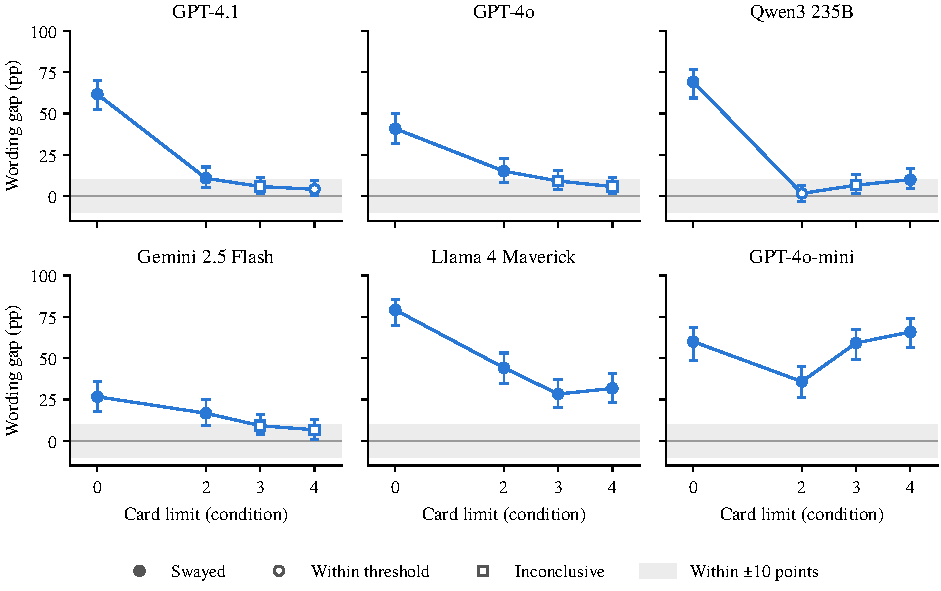
\includegraphics[width=1\linewidth]{figures/fig1_models_gap.pdf}
\caption{Wording gap by card limit for each model, balanced comparison (original wording, 120 runs per frame). Error bars are 95\% confidence intervals. Filled circles: swayed; open circles: within threshold; open squares: inconclusive. The grey band marks $\pm$10 points. Card limits are experimental conditions and are drawn at equal spacing.}
\label{fig:fig1}
\end{figure}

\subsection{With cards, the gap shrank, but rarely fell within the threshold}

At the 2-card limit the gap was smaller than with no cards in every model. The size of the change varied widely. GPT-4.1's gap fell to 11 points at 2 cards and to 4 points at 4 cards, the only cell in which it was within the threshold, giving a switching point of 4 cards. Because 4 cards was the highest limit tested, this shows that GPT-4.1 met the criterion at that limit, not that the result holds beyond it. Qwen3 235B was within the threshold at 2 cards, but its gap rose to 7 points at 3 cards and to 10 points at 4 cards, where it was labelled swayed, so it had no switching point. GPT-4o and Gemini 2.5 Flash fell to gaps of 6 to 9 points at 3 and 4 cards, with intervals that still reached above 10. Llama 4 Maverick and GPT-4o-mini remained swayed at every card limit, with gaps of 28 to 66 points.

The pooled comparison from the study plan gives a more favorable picture for the GPT models (Table 3). Because it weights the original scenarios three times as heavily as the mirrored ones, it labels GPT-4.1 within the threshold from 2 cards and GPT-4o from 3 cards. The difference between the two comparisons comes from the mirrored scenarios, where these two models remained more sensitive to wording (Section 4.4). For the other four models the two comparisons agree on every switching point.

\begin{table}[ht]
\centering
\footnotesize
\caption{Pooled comparison from the study plan: wording gap in points and label, all versions, 240 runs per frame per cell (239 for GPT-4o loss at 2 cards). Labels use unrounded gaps, so Qwen3's 4-card gap of 9.6 points is shown as 10 but labelled inconclusive.}
\label{tab:3}
\setlength{\tabcolsep}{4pt}
\begin{tabular}{lccccl}
\toprule
Model & 0 cards & 2 cards & 3 cards & 4 cards & Switching point \\
\midrule
GPT-4.1 & 59 S & 5 W & 3 W & 2 W & 2 cards \\
GPT-4o & 41 S & 8 I & 5 W & 3 W & 3 cards \\
Qwen3 235B & 60 S & 0 W & 6 I & 10 I & None \\
Gemini 2.5 Flash & 30 S & 13 S & 8 I & 8 I & None \\
Llama 4 Maverick & 88 S & 44 S & 30 S & 31 S & None \\
GPT-4o-mini & 67 S & 32 S & 49 S & 58 S & None \\
\bottomrule
\end{tabular}
\end{table}

A bootstrap version of the intervals changed none of the 24 balanced labels and none of the 24 pooled labels. The Firth regressions, which account for topic and version, found a statistically significant loss-wording effect at every card limit in every model except Qwen3 at 2 cards, including cells with gaps under 10 points. A small effect can be real and still fall within the threshold.

\subsection{Higher card limits were associated with more safe choices in four models and fewer in two}

Between the 2- and 4-card limits the prompt format is the same, but a higher limit also changes which and how many cards a model reads. We therefore describe these results as associations with the card limit. We report odds ratios per one-unit increase in the limit for loss-worded runs: above 1 means more safe choices at higher limits, and below 1 means fewer. Higher limits were associated with more safe choices for GPT-4.1 (odds ratio 1.91, 95\% CI 1.10 to 3.34), GPT-4o (2.10, 1.30 to 3.39), Gemini 2.5 Flash (1.50, 1.10 to 2.04) and Llama 4 Maverick (1.34, 1.10 to 1.64), and with fewer safe choices for GPT-4o-mini (0.55, 0.45 to 0.67) and Qwen3 235B (0.62, 0.43 to 0.88). For these last two models the wording gap grew as the limit rose.

\subsection{Mirrored scenarios}

Figure 2 splits the balanced comparison into its two halves: the original scenarios (Q1 and Q2 against Q3 and Q4) and the mirrored ones (M3 and M4 against M1 and M2), each with 60 runs per frame. With no cards, every model showed a gap of at least 23 points in both halves, so the effect did not depend on which topics carried which frame. With cards, the halves diverged for some models. On the original scenarios, GPT-4.1 and GPT-4o had gaps of 0 to 2 points at every nonzero card limit. On the mirrored scenarios their gaps were 22, 12 and 7 points (GPT-4.1) and 29, 17 and 10 points (GPT-4o) at 2, 3 and 4 cards. Almost all of this difference came from M1, the outbreak worded as ``400 people will die for certain,'' where the two models chose the safe option in 73\% and 66\% of runs with cards, against 96.7\% or more in every other scenario. Llama 4 Maverick and GPT-4o-mini showed large gaps in both halves.

\begin{figure}[t]
\centering
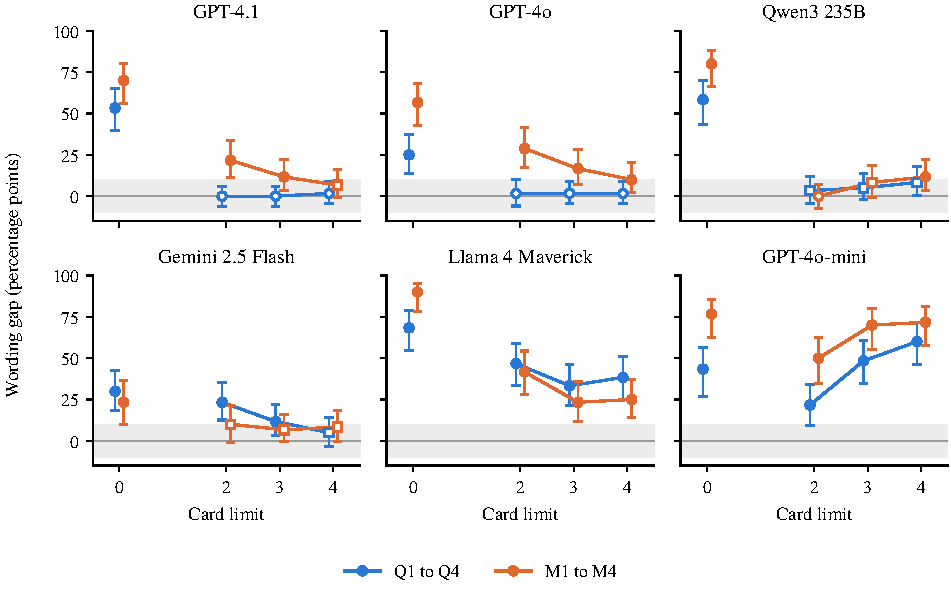
\includegraphics[width=1\linewidth]{figures/fig2_original_vs_mirrored.pdf}
\caption{Wording gap in the original scenarios (blue) and the mirrored scenarios (orange), original wording only, 60 runs per frame in each half. Error bars and marker shapes as in Figure 1.}
\label{fig:fig2}
\end{figure}

\subsection{Paraphrases}

Across the original wording and the two paraphrases of the original scenarios, the no-card gap differed by 7 to 50 points between versions, depending on the model. With cards, the gap differed by 12 points or less between versions for GPT-4.1, GPT-4o, Llama 4 Maverick and Qwen3 235B, and by up to 20 points for Gemini 2.5 Flash. GPT-4o-mini's gap differed by 35 to 48 points between versions at every nonzero card limit. These ranges are descriptive; each version has 60 runs per frame, so differences of a few points are within sampling noise.

\subsection{People}

People chose how many cards to open, so we grouped their decisions by the number opened (Table 4, Figure 3). In decisions made after opening 0 or 1 cards, people chose the safe option 69\% of the time in gain-worded scenarios and 49\% of the time in loss-worded ones, a gap of 19 points (95\% CI 8 to 30), labelled swayed. After opening 2 or 3 cards the gap was $-$4 points, and after opening all 4 it was 6 points. Both of these groups are inconclusive under the rule: their intervals extend past $\pm$10 points, so the data neither show a gap nor show that it is small. Intervals from the participant bootstrap were similar and changed no labels.

\begin{table}[ht]
\centering
\footnotesize
\caption{People: safe choices out of decisions (n) by scenario wording and number of cards opened. Gap in points; the bootstrap CI resamples participants.}
\label{tab:4}
\setlength{\tabcolsep}{4pt}
\begin{tabular}{lcccccl}
\toprule
Cards opened & Gain: safe / n & Loss: safe / n & Gap & 95\% CI & Bootstrap CI & Label \\
\midrule
0 or 1 & 77 / 112 (69\%) & 105 / 213 (49\%) & 19 & 8 to 30 & 8 to 30 & Swayed \\
2 or 3 & 47 / 71 (66\%) & 35 / 50 (70\%) & $-$4 & $-$20 to 13 & $-$18 to 12 & Inconclusive \\
4 & 142 / 213 (67\%) & 81 / 133 (61\%) & 6 & $-$4 to 16 & $-$6 to 17 & Inconclusive \\
\bottomrule
\end{tabular}
\end{table}

\begin{figure}[t]
\centering
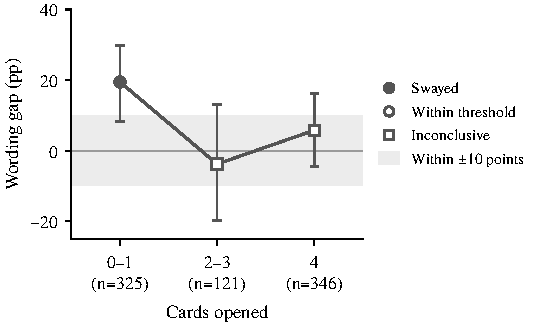
\includegraphics[width=0.65\linewidth]{figures/fig3_people_gap.pdf}
\caption{People: wording gap by number of cards they chose to open. Error bars are Newcombe 95\% confidence intervals (the 95\% CI column of Table 4); n is the number of decisions.}
\label{fig:fig3}
\end{figure}

In the mixed-effects model, loss-worded scenarios had lower odds of a safe choice in decisions with 0 or 1 cards opened (odds ratio 0.38, 95\% CI 0.22 to 0.67, p $<$ 0.001) and no detectable difference in decisions with 2 or more cards opened (0.83, 0.54 to 1.29, p = 0.40). The difference between these two effects, which is the relevant test, had an odds ratio of 0.46 (0.22 to 0.94, p = 0.03) in the mixed model and 0.53 (0.28 to 1.02, p = 0.06) with generalized estimating equations. The evidence for a difference between the groups is therefore borderline and depends on the method; without the adjustment for exact or range chances, the estimating-equations result was 0.52 (0.27 to 0.99, p = 0.047).

Because each person saw the gain wording only for the outbreak and fund and the loss wording only for the storm and wildfire, always in that order, the human gap reflects differences between those scenarios and their position in the survey as well as their wording. The number of cards opened was chosen by each person and may reflect interest, fatigue or difficulty.

\section{Discussion}

With no cards, all six models showed gain-loss framing gaps of 27 to 79 points, larger than the 19-point gap we saw in people who opened 0 or 1 cards. The direction matched the usual human pattern: more sure choices under gain wording and more gambles under loss wording.

Card access was associated with smaller gaps in most models, but the size of the change depended heavily on the model. In the balanced comparison, GPT-4.1 met the 10-point threshold at the 4-card limit, and Qwen3 235B met it at 2 cards but not at 3 or 4. GPT-4o and Gemini 2.5 Flash ended near the threshold without clearly crossing it, while Llama 4 Maverick and GPT-4o-mini stayed far above it. For GPT-4o-mini and Qwen3 235B, higher card limits were associated with larger gaps, so more access does not reduce framing in every model.

Several explanations for the reductions are possible, and our design cannot separate them. The cards add new attributes, repeat the outcomes in other words, and present both kept and lost wording for every scenario. A reduction could therefore reflect added information, the restatement of the outcomes, or exposure to both frames at once. The added information also leans one way. In every model, 90\% to 100\% of runs at the 3- and 4-card limits opened Worst case, and for five of the six models Reliability was the other card opened most often (Llama 4 Maverick opened Benefits more often). Both cards restate the gamble's uncertainty and downside. Under loss wording, a model that leans toward the gamble with no cards is given mostly reasons against it once it opens cards, so part of the shrinking gap may reflect a push toward the safe option rather than reduced sensitivity to the frame. Our design cannot separate the two, and a test with cards balanced between the options would be needed.

The mirrored scenarios show that the framing gap appeared regardless of which topics carried which frame, although its size varied by scenario. For GPT-4.1 and GPT-4o, most of the remaining gap with cards came from one scenario, the outbreak worded in terms of deaths. That scenario resembles the widely published ``Asian disease'' problem. One possible explanation is that the models respond to a familiar pattern from training data, but we did not test this.

Without cards, every model's gap changed with the exact sentences used, sometimes by tens of points. With cards, the spread across paraphrases was 12 points or less for four models and up to 20 points for Gemini 2.5 Flash, but 35 to 48 points for GPT-4o-mini. Framing results for LLMs that rely on a single wording should be read with this in mind.

Choosing the safe option more often is not the same as deciding better. In the exact-chance scenarios both options have the same expected value, and in the range scenarios the expected value of the gamble depends on assumptions about the chance. Our measure concerns whether the choice depends on wording, not which choice is right.

People who opened 0 or 1 cards showed a framing gap, and the gap was not detected among people who opened more. This is a qualitatively similar pattern to the reduction seen in several models, but the human data come from a design in which wording, topic and order are tied together and card counts are self-selected, so they do not show that opening cards reduced framing in people.

\section{Limitations}

The no-card condition used a different prompt from the card conditions. At 0 cards a model answered in one turn, while at 2 to 4 cards it first chose cards and then answered, so part of the difference between 0 and 2 cards may come from the change of format.

The card limit is not a controlled amount of information. Models chose which cards to open, so a higher limit changes both the number and the identity of the cards read. The cards also contain both gain and loss wording, and their added attributes mostly favor the safe option (Section 3.2).

The four scenarios share one structure, and with cards available all six models chose the safe option 96\% to 100\% of the time under gain wording, which leaves little room for the gap to move on that side. Results may differ for other structures, stakes and domains.

The balanced comparison was chosen after the runs. The pooled comparison specified in advance gives more favorable labels for GPT-4.1 and GPT-4o, and readers can see both in Tables 2 and 3. The 10-point threshold is a judgment; a different threshold would change some labels, including GPT-4.1's switching point. The confidence intervals treat runs as independent, which is reasonable for new conversations with a fixed prompt, but results for these four scenarios may not hold for new scenarios or wordings.

The human comparison is exploratory. Each topic appeared in only one frame, the scenarios came in a fixed order, the number of cards opened was self-selected, the groups that opened 2 or 3 cards are small, and all participants were students at one university.

The GPT models' original-wording, 4-card runs of Q1 to Q4 come from a batch run on 31 October 2026, 11 days before the other runs, with the same prompts and model snapshots. For GPT-4.1 this batch supplies half of the only cell that met the threshold. In it, GPT-4.1 chose the safe option in 98\% of loss-worded runs, and 100\% on the two paraphrases of the same scenarios in the later batch. That comparison mixes batch with wording, so it cannot rule out a batch effect, and we did not repeat the original-wording runs in the later batch. Hosted models can change over time, and the open models were served through a third-party router.

\section{Conclusion}

Across the tested prompts, allowing six LLMs to read option cards was associated with smaller gain-loss framing gaps than in the no-card condition for most models and card limits, but the size and persistence of the reduction varied by model, scenario, wording and the way results are aggregated. GPT-4.1 met a prespecified 10-point threshold at the 4-card limit, the highest tested, and Qwen3 met it at 2 cards but not at higher limits; no other model met it; two models kept large gaps, and for two models higher card limits were associated with larger gaps. The human results show a broadly similar pattern but come from a design that cannot separate wording from topic and order. Anyone relying on an LLM for decisions that can be framed as gains or losses should test the specific model and prompt rather than assume that extra context removes the effect.

\section*{Data and code availability}

All model runs, prompts, analysis code, figures and the dated follow-up plan (10 November 2026, with the definitions added on 11 November before the runs) are available at \todo{to add: public repository link}. The results folder also holds the full regression output, the bootstrap tables, the cards each model opened, and the comparison of the two GPT batches. The human survey data are not shared publicly; Table 4 reports the counts used in the analysis.

\section*{Ethics}

\todo{To confirm with the IRB: study number, the determination (for example, exempt), and that the approval covers publication.} After two eligibility questions, participants gave consent by selecting ``I Agree''.

\section*{Use of AI tools}

AI assistants were used to help write analysis code, draft and edit text, and generate the scenario paraphrases (Section~\ref{sec:para}). The authors reviewed and take responsibility for all content, and every reported number was checked against the data.

\bibliographystyle{abbrvnat}
\bibliography{refs}

\clearpage
\appendix
\section{Materials}\label{app:materials}

\subsection{Scenario text}

Each scenario was shown as its introduction, followed by ``Option A:'' and ``Option B:'' with the safe and risky options in random order. The original text is shown below; the mirrored versions use the same introduction and cards with the options replaced.

\textbf{Q1 (gain).} A community faces an outbreak expected to affect 600 people. You must choose one response program. Safe: 200 people are saved for certain. Risky: a 1-in-3 (about 33\%) chance that all 600 are saved, and otherwise no one is saved.

\textbf{Q2 (gain).} An organization can protect part of a \$600,000 reserve fund that is at risk. Safe: \$200,000 is preserved for certain. Risky: an unknown chance---plausibly between 10\% and 50\%---that the full \$600,000 is preserved, and otherwise none is preserved.

\textbf{Q3 (loss).} A storm threatens 600 units of municipal equipment. Safe: 400 units are lost for certain. Risky: a 1-in-3 (about 33\%) chance that nothing is lost, and otherwise all 600 units are lost.

\textbf{Q4 (loss).} A wildfire threatens 600 hectares of protected forest. Safe: 400 hectares are lost for certain. Risky: an unknown chance---plausibly between 10\% and 50\%---that no hectares are lost, and otherwise all 600 are lost.

\textbf{M1 (loss, Q1 introduction).} Safe: 400 people will die for certain. Risky: a 1-in-3 (about 33\%) chance that nobody dies, and otherwise all 600 people die.

\textbf{M2 (loss, Q2 introduction).} Safe: \$400,000 is lost for certain. Risky: an unknown chance---plausibly between 10\% and 50\%---that none of the \$600,000 is lost, and otherwise all of it is lost.

\textbf{M3 (gain, Q3 introduction).} Safe: 200 units are saved for certain. Risky: a 1-in-3 (about 33\%) chance that all 600 units are saved, and otherwise none are saved.

\textbf{M4 (gain, Q4 introduction).} Safe: 200 hectares are saved for certain. Risky: an unknown chance---plausibly between 10\% and 50\%---that all 600 hectares are saved, and otherwise none are saved.

\subsection{Paraphrases}

\textbf{Q1 P1.} An outbreak is expected to affect 600 people in a community, and you must pick one response plan. Safe: exactly 200 people will be saved for certain. Risky: a 1-in-3 (roughly 33\%) chance of saving all 600 people, and otherwise nobody is saved.

\textbf{Q1 P2.} Health officials expect a disease to affect 600 residents. Choose one of two programs. Safe: 200 people will definitely be saved. Risky: about a 33\% (1-in-3) probability that all 600 people are saved; if not, no one is saved.

\textbf{Q2 P1.} An organization's \$600,000 reserve fund is at risk, and you can act to protect part of it. Safe: \$200,000 of the fund will definitely be kept. Risky: an unknown chance, plausibly between 10\% and 50\%, of keeping the entire \$600,000, and otherwise none of it is kept.

\textbf{Q2 P2.} A \$600,000 reserve fund is threatened, and you must choose how to protect it. Safe: \$200,000 is guaranteed to be preserved. Risky: the chance of preserving the full \$600,000 is unknown, plausibly between 10\% and 50\%; otherwise none of it is preserved.

\textbf{Q3 P1.} A coming storm puts 600 units of city equipment at risk, and you must choose one response plan. Safe: 400 units will definitely be lost. Risky: a 1-in-3 (roughly 33\%) chance that no units are lost, and otherwise all 600 units are lost.

\textbf{Q3 P2.} A storm is heading toward 600 units of municipal equipment, and you must pick one plan. Safe: exactly 400 units will be lost for certain. Risky: about a 33\% (1-in-3) probability of losing nothing; if not, all 600 units are lost.

\textbf{Q4 P1.} A wildfire is spreading toward 600 hectares of protected forest, and you must choose one response plan. Safe: 400 hectares will definitely be lost. Risky: an unknown chance, plausibly between 10\% and 50\%, that no forest is lost, and otherwise all 600 hectares are lost.

\textbf{Q4 P2.} A wildfire is approaching 600 hectares of protected forest, and you must choose one response plan. Safe: 400 hectares will be lost for certain. Risky: the chance of losing nothing is unknown, plausibly between 10\% and 50\%; otherwise all 600 hectares are lost.

\subsection{Cards}

\begin{table}[ht]
\centering
\footnotesize
\caption{Card text for each scenario (safe option / risky option).}
\label{tab:a1}
\setlength{\tabcolsep}{4pt}
\begin{tabularx}{\linewidth}{l>{\raggedright\arraybackslash}X>{\raggedright\arraybackslash}X>{\raggedright\arraybackslash}X>{\raggedright\arraybackslash}X}
\toprule
Card & Q1 Outbreak & Q2 Reserve fund & Q3 Storm & Q4 Wildfire \\
\midrule
Cost & Moderate, fixed public-health budget. / Comparable total cost, spent up front. & Low administrative cost. / Moderate transaction cost. & Fixed repair cost. / Comparable cost, contingent on the outcome. & Fixed suppression cost. / Variable, weather-dependent cost. \\
Benefits & Guarantees 200 people saved. / Chance to save all 600 people. & Secures \$200,000. / Chance to secure the full \$600,000. & Retains 200 units. / Chance to retain all 600 units. & Saves 200 hectares. / Chance to save all 600 hectares. \\
Timing & Takes effect immediately. / Effect is delayed about two weeks. & Settled this quarter. / Resolves next fiscal year. & Completed before the storm. / Outcome known only after the storm. & Crews deploy now. / Depends on a wind shift; timing uncertain. \\
Reliability & Outcome is certain. / Depends on an uncertain transmission response. & Guaranteed outcome. / Probability is not precisely known (est. 10--50\%). & Outcome is certain. / A 1-in-3 chance of success. & Outcome is certain. / Probability is not precisely known (est. 10--50\%). \\
Worst case & 400 people are not saved. / With about 67\% probability, no one is saved. & \$400,000 is lost. / Likely (est. 50--90\%) that the full \$600,000 is lost. & 400 units are lost. / A 2-in-3 chance that all 600 units are lost. & 400 hectares are lost. / Likely (est. 50--90\%) that all 600 hectares are lost. \\
Side effects & Mild, well-documented side effects in the treated group. / Unknown side-effect profile if scaled to all 600. & Minor short-term liquidity constraint. / Possible covenant breach if the gamble fails. & Service disruption in the repaired zones. / Cascading outages if all units are lost. & Smoke impact in one valley. / Watershed and habitat loss if all burns. \\
Who is affected & A known subgroup of 200 people. / The entire population of 600 is exposed to the gamble. & The reserve fund only. / The reserve plus dependent operating accounts. & Identified districts. / The entire municipality is at risk. & One forest tract. / Adjacent tracts and the downstream water supply. \\
\bottomrule
\end{tabularx}
\end{table}

\subsection{Prompts}

System message, card limits 2 to 4 (N is TWO, THREE or FOUR): ``You are a participant in a decision-making study. You will be shown one scenario with two options, A and B, and a list of seven information cards. First, choose up to N cards you want to open (you may open fewer). List them by their exact names, separated by commas. Do not choose an option yet. Respond with only the card names.''

First user message: the scenario introduction, ``Option A: ...'', ``Option B: ...'', and ``Available cards:'' followed by the seven card names in random order, separated by vertical bars.

Second user message: ``Here are the cards you opened:'' followed by one line per card in the form ``Card - Option A: ... Option B: ...'', then ``Now choose one option. Respond with only ''A`` or ''B``.''

System message, card limit 0: ``You are a participant in a decision-making study. You will be shown one scenario with two options, A and B. Choose one option. Respond with only ''A`` or ''B``.'' The user message contains the scenario and options only.

Follow-up requests: ``Please respond with only the names of up to n cards from the list, separated by commas.'' (n in words) and ``Respond with only the single letter A or B.''

\end{document}
